\documentclass[10pt]{article}
\usepackage[margin=0.85in]{geometry}
\usepackage{amsmath,amssymb,booktabs,graphicx}
\graphicspath{{figures/}}
\setlength{\parindent}{0pt}
\setlength{\parskip}{5pt}
\newcommand{\E}{\mathbb{E}}
\newcommand{\Var}{\operatorname{Var}}
\newcommand{\Cov}{\operatorname{Cov}}



\begin{document}

\section*{Problem 1: Poisson estimation}
Let $S=\sum_{i=1}^N x_i$, with $N>0$. Use the shape--rate convention
\[
p(\lambda)=\frac{b^a}{\Gamma(a)}\lambda^{a-1}e^{-b\lambda},\qquad a,b>0.
\]
If $b$ is instead the Gamma scale, replace $b$ by $1/b$ in the results below.
\subsection*{(a) Joint likelihood}
Independence gives
\[
L(\lambda;\mathbf{x})=\prod_{i=1}^N\frac{\lambda^{x_i}e^{-\lambda}}{x_i!}
=\frac{\lambda^S e^{-N\lambda}}{\prod_{i=1}^N x_i!}.
\]
\subsection*{(b) Maximum likelihood}
\begin{align*}
\ell(\lambda)&=S\log\lambda-N\lambda-\sum_{i=1}^N\log(x_i!),\\
\ell'(\lambda)&=\frac{S}{\lambda}-N, &
\ell''(\lambda)&=-\frac{S}{\lambda^2}.
\end{align*}
For $S>0$, setting the derivative to zero yields the unique maximum
\[\lambda_{\mathrm{ML}}=\frac{S}{N}.\]
If $S=0$, the likelihood decreases with $\lambda$. Its maximum is at zero if the boundary is allowed; on a strictly positive parameter space, there is only a supremum as $\lambda\downarrow0$.
\subsection*{(c) Maximum a posteriori}
\begin{align*}
\log p(\lambda\mid\mathbf{x})&=C+(S+a-1)\log\lambda-(N+b)\lambda,\\
\frac{d}{d\lambda}\log p(\lambda\mid\mathbf{x})&=\frac{S+a-1}{\lambda}-(N+b).
\end{align*}
For $S+a>1$, the second derivative is negative and
\[\lambda_{\mathrm{MAP}}=\frac{S+a-1}{N+b}.\]
For $S+a=1$ the density decreases; for $S+a<1$ it diverges near zero. The boundary mode is conventionally reported as zero, with the strictly positive domain qualification above.
\subsection*{(d) Posterior distribution}
Bayes' rule gives
\[
p(\lambda\mid\mathbf{x})\propto L(\lambda;\mathbf{x})p(\lambda)
\propto\lambda^{S+a-1}e^{-(N+b)\lambda}.
\]
Normalizing this Gamma kernel,
\[
p(\lambda\mid\mathbf{x})=\frac{(N+b)^{S+a}}{\Gamma(S+a)}\lambda^{S+a-1}e^{-(N+b)\lambda},
\qquad \lambda\mid\mathbf{x}\sim\operatorname{Gamma}(S+a,N+b).
\]
\subsection*{(e) Posterior mean and variance}
\[
\E[\lambda\mid\mathbf{x}]=\frac{S+a}{N+b},\qquad
\Var(\lambda\mid\mathbf{x})=\frac{S+a}{(N+b)^2}.
\]
The mean can be written as
\[
\E[\lambda\mid\mathbf{x}]=\frac{N}{N+b}\lambda_{\mathrm{ML}}+\frac{b}{N+b}\frac{a}{b}.
\]
It averages the sample mean and prior mean $a/b$. For an interior mode, the mean exceeds $\lambda_{\mathrm{MAP}}$ by $1/(N+b)$. With fixed $a,b$, increasing $N$ makes the prior influence vanish; the mean and mode approach the MLE, and the variance decreases when the sample mean remains bounded.
\clearpage
\section*{Problem 2: Ridge regression}
Condition on $X$ and write $y=Xw+\varepsilon$, where $w$ is fixed,
$\E[\varepsilon\mid X]=0$, and $\Cov(\varepsilon\mid X)=\sigma^2I_n$.
Let $A=X^TX+\lambda I_d$. At $\lambda=0$, inverse formulas require full column rank.
\subsection*{(a) Mean and covariance}
\begin{align*}
w_{\mathrm{RR}}&=A^{-1}X^Ty
=A^{-1}X^TXw+A^{-1}X^T\varepsilon,\\
\E[w_{\mathrm{RR}}\mid X]&=A^{-1}X^TXw
=A^{-1}(A-\lambda I)w
=(I-\lambda A^{-1})w.
\end{align*}
Thus the bias is $-\lambda A^{-1}w$. Since $A$ is symmetric,
\begin{align*}
\Cov(w_{\mathrm{RR}}\mid X)
&=A^{-1}X^T\Cov(\varepsilon\mid X)X(A^{-1})^T\\
&=\sigma^2 A^{-1}X^TXA^{-1}.
\end{align*}
This is a $d\times d$ covariance matrix. At $\lambda=0$, the mean is $w$ and the covariance is $\sigma^2(X^TX)^{-1}$.
To express the covariance in an equivalent form, write $B=X^TX$ and
\[
Z=(I+\lambda B^{-1})^{-1}=(B+\lambda I)^{-1}B=A^{-1}B.
\]
Since $Z^T=BA^{-1}$,
\[
\sigma^2 ZB^{-1}Z^T=\sigma^2 A^{-1}BB^{-1}BA^{-1}
=\sigma^2 A^{-1}BA^{-1}=\Cov(w_{\mathrm{RR}}\mid X).
\]
Thus the derived covariance is exactly $\sigma^2 Z(X^TX)^{-1}Z^T$.
\subsection*{(b) Ridge as shrinkage of least squares}
For full column rank, let $X=USV^T$ be the thin SVD, with
$S=\operatorname{diag}(s_1,\ldots,s_d)$ and $U^TU=V^TV=I$.
\begin{align*}
X^TX&=VS^2V^T,\\
X^TX+\lambda I&=V(S^2+\lambda I)V^T,\\
(X^TX+\lambda I)^{-1}&=V(S^2+\lambda I)^{-1}V^T,\\
w_{\mathrm{LS}}&=(X^TX)^{-1}X^Ty=VS^{-1}U^Ty,\\
V^Tw_{\mathrm{LS}}&=S^{-1}U^Ty,\\
U^Ty&=SV^Tw_{\mathrm{LS}}.
\end{align*}
Substituting the final equality into the ridge solution,
\begin{align*}
w_{\mathrm{RR}}&=V(S^2+\lambda I)^{-1}SU^Ty\\
&=V(S^2+\lambda I)^{-1}S^2V^Tw_{\mathrm{LS}}\\
&=\sum_{j=1}^d\frac{s_j^2}{s_j^2+\lambda}\,v_j(v_j^Tw_{\mathrm{LS}}).
\end{align*}
The component along $v_j$ is shrunk by $s_j^2/(s_j^2+\lambda)$, so smaller singular values receive stronger shrinkage. In this basis,
\[
\Cov(w_{\mathrm{RR}}\mid X)=\sigma^2V\operatorname{diag}\!\left(\frac{s_j^2}{(s_j^2+\lambda)^2}\right)V^T.
\]
For rank-deficient $X$, use the compact rank-$r$ SVD and $w_{\mathrm{LS}}=X^+y$; the same sum over positive singular values holds for $\lambda>0$. Null-space components are zero in both ridge and minimum-norm least squares.
\clearpage
\section*{Problem 3, Part 1: Linear regression}
The four CSV files were extracted from the supplied ZIP. The training and test feature matrices have sizes $350\times7$ and $42\times7$. Column 7 is the constant one. The supplied linear columns are retained, and all seven coefficients, including the intercept, are penalized as specified. Part 1 is implemented in \texttt{question3.py}, using only training observations to solve
\[
L(w)=\lambda\|w\|_2^2+\sum_{i=1}^{350}(y_i-x_i^Tw)^2.
\]
The stationarity condition gives $(X^TX+\lambda I)w=X^Ty$. Test data are used only for the requested prediction error evaluation in (c).
\subsection*{(a) Coefficient paths}
Using the training SVD,
\begin{align*}
w(\lambda)&=V\operatorname{diag}\!\left(\frac{s_j}{s_j^2+\lambda}\right)U^Ty,\\
H(\lambda)&=X(X^TX+\lambda I)^{-1}X^T,\\
\operatorname{df}(\lambda)&=\operatorname{tr}H(\lambda)=\sum_j\frac{s_j^2}{s_j^2+\lambda}.
\end{align*}
Every integer $\lambda=0,\ldots,5000$ is evaluated. At zero, the SVD pseudoinverse gives least squares. Increasing $\lambda$ decreases degrees of freedom; individual coefficients need not vary monotonically.
\begin{center}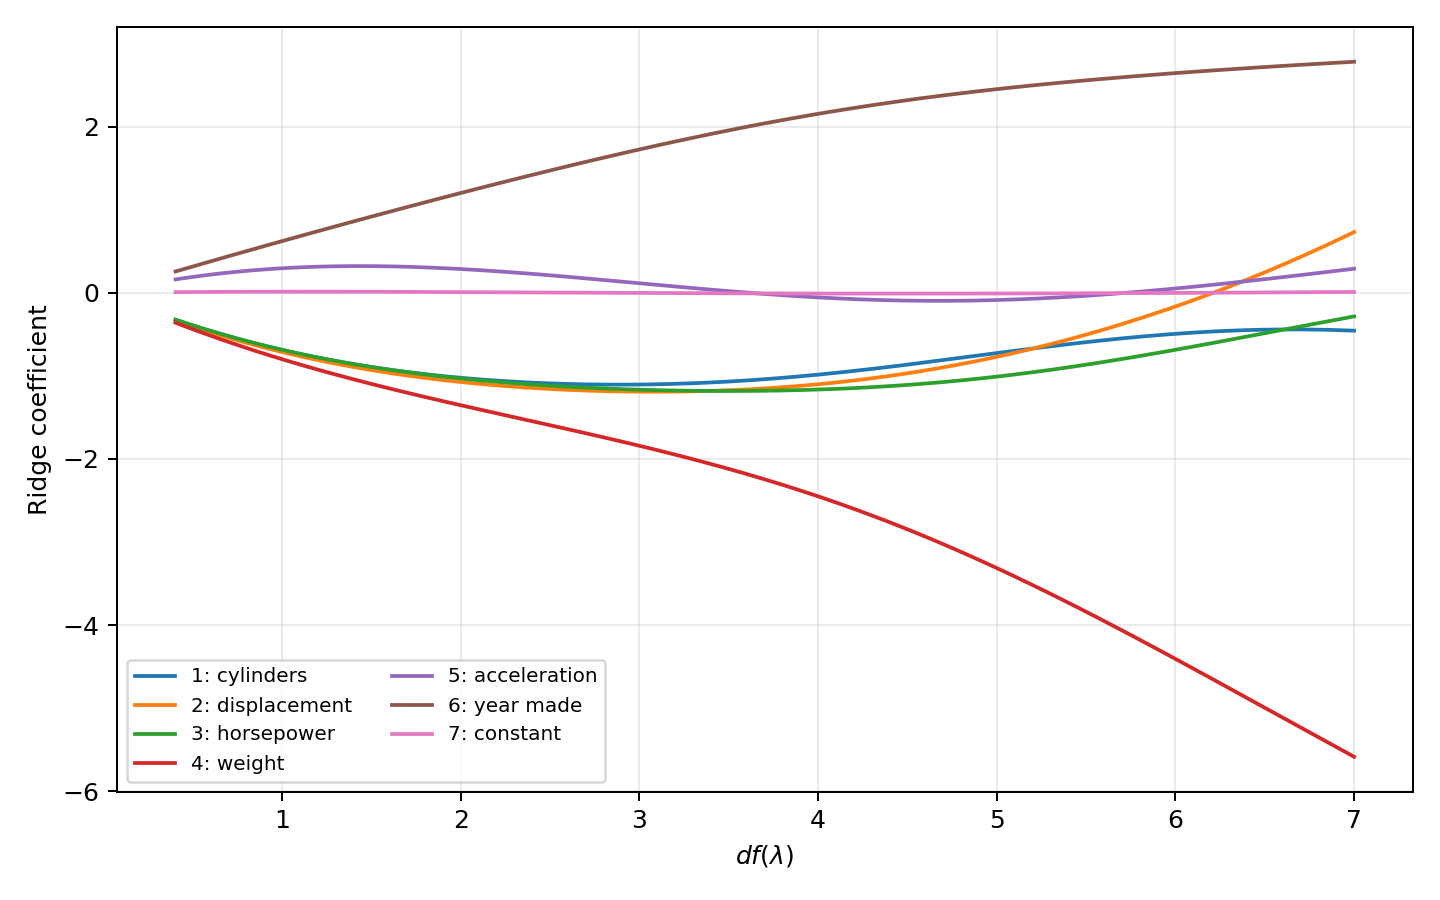
\includegraphics[width=0.70\linewidth]{a_coefficients_vs_df.png}\end{center}
\subsection*{(b) Outstanding dimensions}
Dimensions 4 (weight) and 6 (year made) stand out. At $\lambda=0$, their coefficients are $-5.58558$ and $+2.78140$; the remaining magnitudes are below $0.74$. Holding the other predictors fixed, higher standardized weight predicts lower mpg and later year predicts higher mpg. These are conditional predictive associations, not causal effects. Correlated features also limit interpretation based on coefficient magnitude alone.
The least squares vector, in input order, is
\[
w_{\mathrm{LS}}=\begin{bmatrix}-0.456272&0.730192&-0.284648&-5.585580&0.289570&2.781398&0.010156\end{bmatrix}^T.
\]
\clearpage
\subsection*{(c) Linear-model test RMSE}
For every $\lambda=0,\ldots,50$, predict all 42 test cases using
\[
\widehat y_{\mathrm{test}}=X_{\mathrm{test}}w(\lambda),\qquad
\operatorname{RMSE}(\lambda)=\sqrt{\frac1{42}\sum_{i=1}^{42}(y_{\mathrm{test},i}-\widehat y_{\mathrm{test},i})^2}.
\]
\begin{center}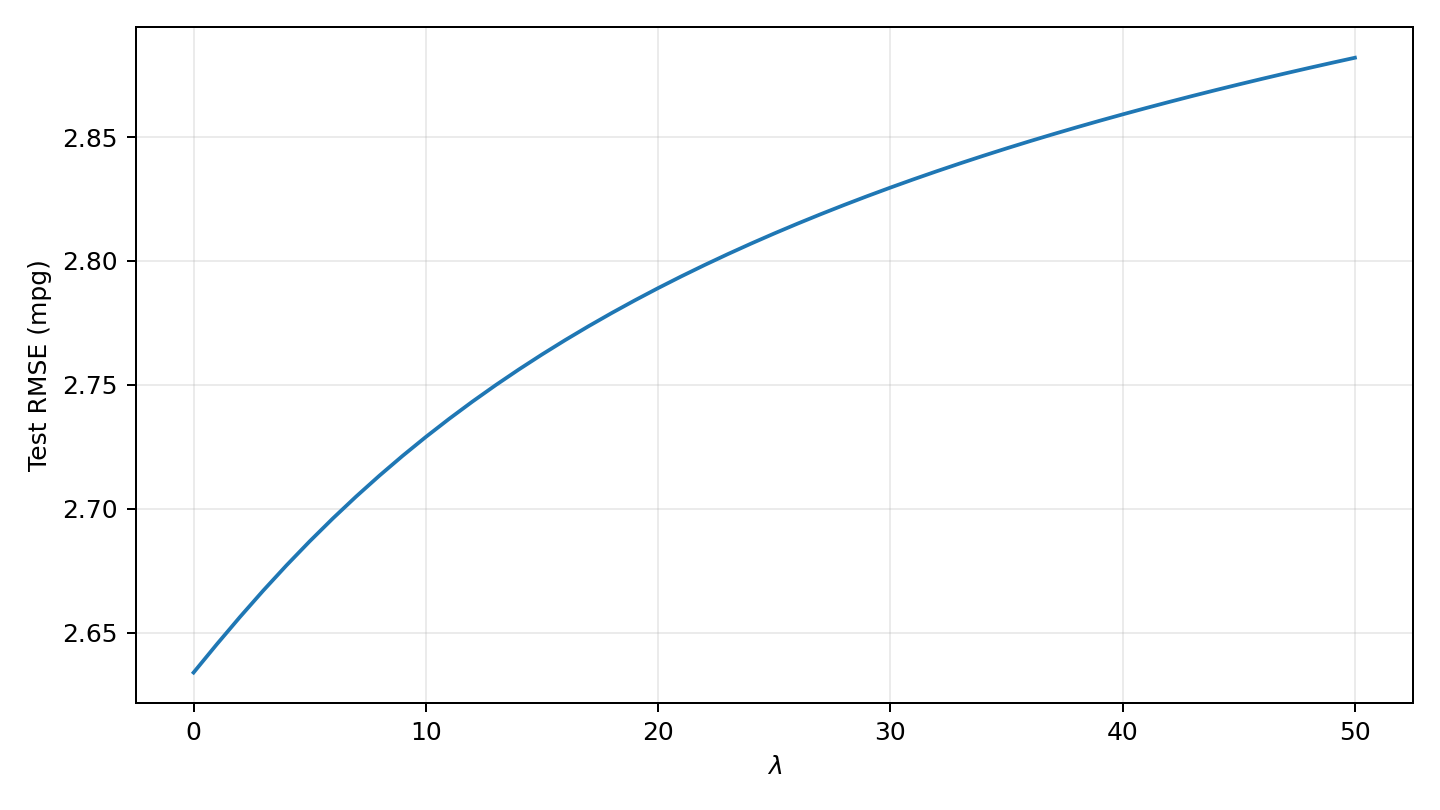
\includegraphics[width=0.72\linewidth]{c_rmse_vs_lambda.png}\end{center}
The minimum on the requested grid is at $\lambda=0$: RMSE $=2.633889$ mpg. Error increases with $\lambda$ on this grid. Thus least squares is preferred for the linear model on these test observations; positive shrinkage does not improve its observed prediction error.
\clearpage
\section*{Problem 3, Part 2: Polynomial regression}
\subsection*{(d) Construction and test comparison}
Part 2 is implemented in \texttt{question3.py}, where the Part 2 section expands the design matrix and reuses the shared SVD ridge solver. Use separate powers of each feature, without interactions:
\[
\phi_p(x)=\bigl[x_1,\ldots,x_6,\widetilde{x_1^2},\ldots,\widetilde{x_6^2},\ldots,
\widetilde{x_1^p},\ldots,\widetilde{x_6^p},1\bigr]^T.
\]
For $p=1$, only the supplied linear columns and intercept are used. The expansion uses separate powers, with no interaction terms and $6p+1$ columns. Each added column $z$ is standardized using the empirical standard deviation formula, with statistics fitted on training data only:
\[
\mu_z=\frac1{350}\sum_i z_i,\qquad
s_z=\sqrt{\frac1{350}\sum_i(z_i-\mu_z)^2},\qquad
\widetilde z=\frac{z-\mu_z}{s_z}.
\]
The same $\mu_z,s_z$ transform test columns. The intercept remains one. Fit ridge for each $p=1,2,3$ and integer $\lambda=0,\ldots,100$.
\begin{center}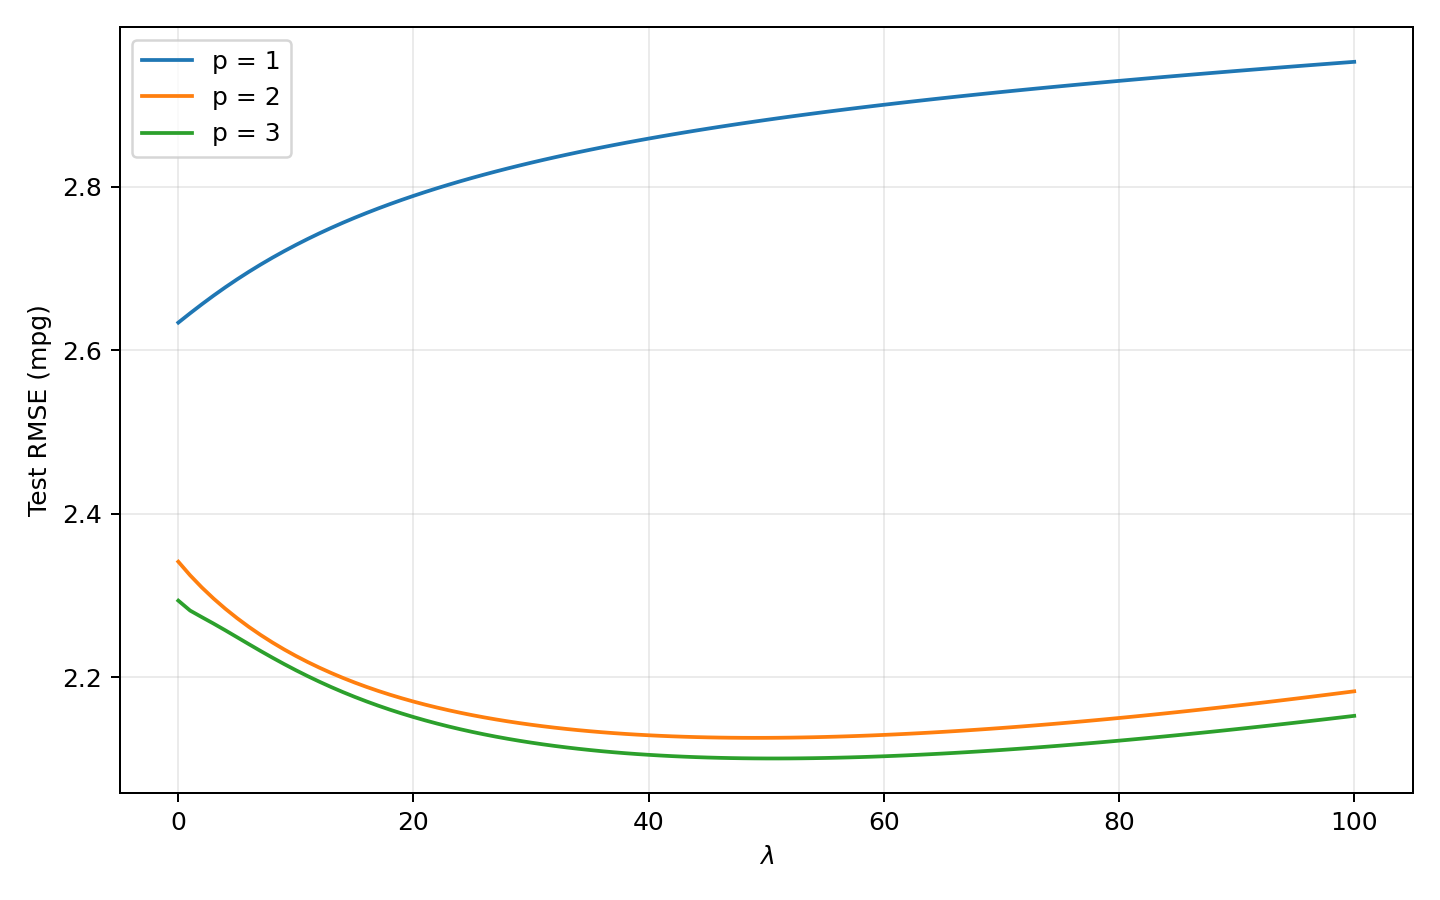
\includegraphics[width=0.72\linewidth]{d_rmse_vs_lambda.png}\end{center}
\subsection*{Model choice}
\begin{center}
\begin{tabular}{ccccc}
\toprule
$p$ & Coefficients & Best $\lambda$ & Best RMSE & RMSE at $\lambda=0$\\
\midrule
1 & 7 & 0 & 2.633889 & 2.633889\\
2 & 13 & 49 & 2.125536 & 2.341201\\
3 & 19 & 51 & 2.100297 & 2.293523\\
\bottomrule
\end{tabular}
\end{center}
Choose $p=3$ based on the requested test comparison, since its minimum error is smallest, at $\lambda=51$. Its advantage over $p=2$ is modest: about $0.02524$ mpg (1.19\% of the quadratic RMSE). This plot alone does not establish that the small difference will persist on new data.

The preferred penalty changes from zero for the linear model to around 50 for the polynomial models. Added powers increase flexibility and create correlated columns; shrinkage improves test performance here. For $p=3$, regularization reduces RMSE from $2.293523$ to $2.100297$ mpg. The numerical penalty depends on scaling and the sum-of-squares loss, so it is not directly transferable to other formulations.

These choices describe the supplied test comparison as requested. In a fresh predictive evaluation, choose $p$ and $\lambda$ by validation or cross-validation within the training data, then evaluate on an untouched holdout set.
\end{document}
